\chapter{Literature survey}\label{chap:Lit}

\section{Operational amplifiers}\label{sec:opamps}

\subsubsection{Operational amplifiers: limitations and considerations}\label{sec:opamps_limits}
There are many practical limitations to operational amplifiers in comparison to the ideal model. The limit on the common mode voltage is a concern as the limit is usually around the rail voltage and since the negative rail will be ground and the common mode voltage will be close to 0 the data sheet should be consulted to ensure normal operation of the op amp \cite{NonIdeal_Opamps}. 

A significant consideration is the offset voltage between the inputs of the opamp as when the inputs are equal (no current is being given to the load) there will be an offset voltage on the order of mV which is a similar magnitude to the relevant voltages \cite{Lim_Opamps}. This will result in significant output voltages at no load. However a negative feedback will greatly reduce the impact of input offset voltage and current \cite{Lim_Opamps}.

The output voltage won't be able to go all the way to the rail voltages. Therefore there will be some output voltage when there is no current through the load due to the output not able to go below a certain voltage above ground.
\subsubsection{Operational amplifier configurations}\label{sec:opamps_configs}
There are many different configurations for operational amplifiers, this section will cover 4 basic configurations that could be useful for the current sensor.

The simplest circuit is the voltage follower, it requires no other components and causes the output voltage to track the input voltage. The op amp in this configuration provides a large input impedance and very low output impedance which can allow signals to pass between logic components without them loading each other and can be used to stabilize a voltage divider \cite{Fund_Opamps}.

The inverting op amp is a configuration where the output is connected to the inverting input terminal using a resistor, there is a second resistor connecting this terminal to the circuit input. The non-inverting input is connected to ground. This configuration results in a gain equal to the negative of the ratio between the two resistors. The negative gain cause the output to be exactly out of phase with the input \cite{Fund_Opamps}.

The non-inverting op amp configuration is similar to the inverting amplifier except the input is connected directly to the non-inverting input and the inverting input terminal has a resistor connecting it to the ground. This results in the gain being equal to 1 plus the ratio between the two resistors \cite{Fund_Opamps}.

The differential amplifier is similar to the inverting amplifier, but instead of connecting the non-inverting input to ground a second signal is connected to the input of this terminal through a resistor of the same value  as the other terminal. This results in the output being the difference between the two signals scaled by the ratio of the feedback resistor to the input resistor. This configuration is good at filtering out noise common to both input terminals \cite{Fund_Opamps}. 

\begin{figure}[H]
\footnotesize
\centering
\begin{subfigure}[]{0.45\textwidth}
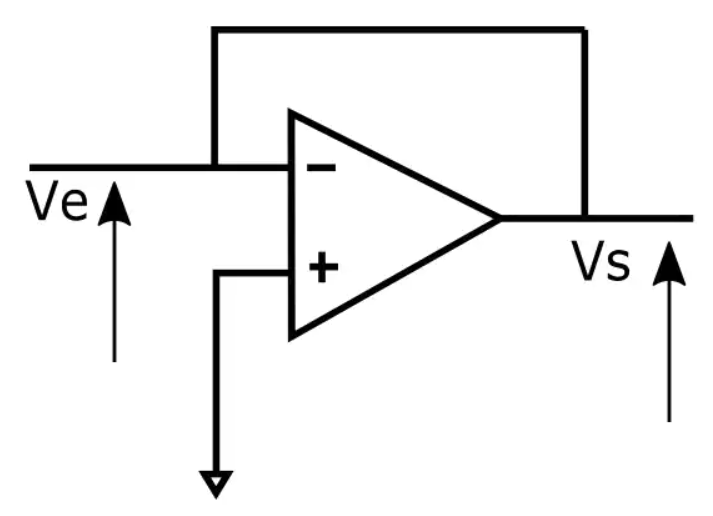
\includegraphics[width=\linewidth]{./Figures/Follower.png}
\caption{Circuit diagram for a voltage follower\cite{Fund_Opamps}}
\label{subfig:opamp_foll}	
\end{subfigure}
\begin{subfigure}[]{0.45\textwidth}
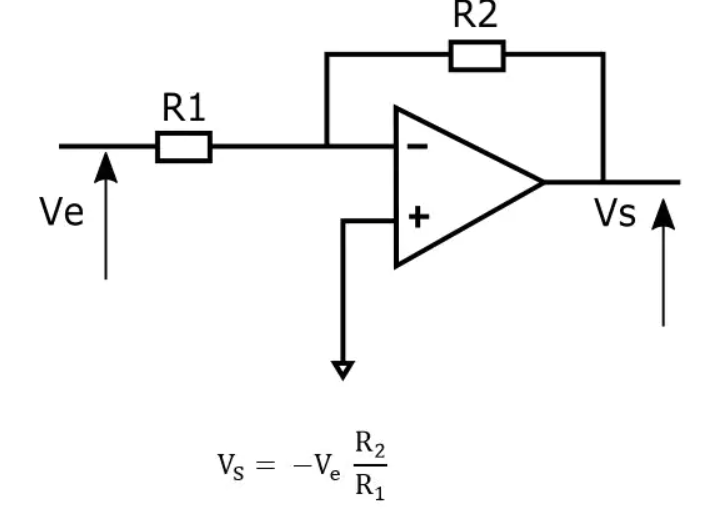
\includegraphics[width=\linewidth]{./Figures/Inverting.png}
\caption{Circuit diagram for a inverting op amp \cite{Fund_Opamps}.} 			
\label{subfig:opamp_invert}	
\end{subfigure}
\begin{subfigure}[]{0.45\textwidth}
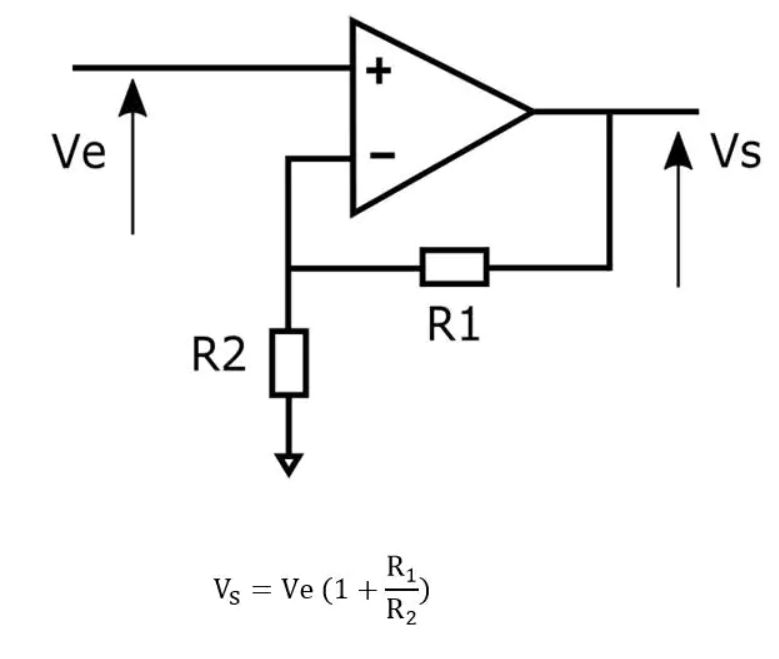
\includegraphics[width=\linewidth]{./Figures/NonInverting.png}
\caption{Circuit diagram for a non-inverting op amp \cite{Fund_Opamps}}
\label{subfig:opamp_noninvert}	
\end{subfigure}
\begin{subfigure}[]{0.45\textwidth}
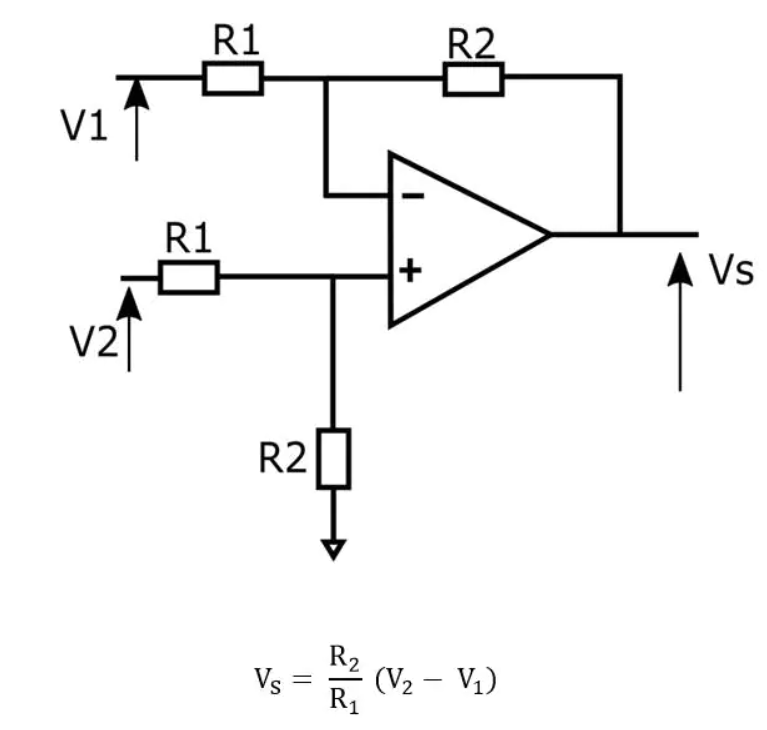
\includegraphics[width=\linewidth]{./Figures/Differential.png}
\caption{Circuit diagram for a differential op amp \cite{Fund_Opamps}} 			
\label{subfig:opamp_dif}	
\end{subfigure}
\caption {Circuit diagrams of 4 op amp configurations}.
\label{fig:circuit_diagram}
\end{figure}

\newpage
\section{Current sensing}\label{sec:cursens}
There are many different techniques to measure current. Both invasive and non invasive methods each with their own advantages and disadvantages that make them suitable for different situations. An invasive current sensor negatively affect the system and decreases performance whereas a non-invasive current sensor doesn't affect the operation of the system at a meaningful level. 

\subsubsection{Hall effect}\label{sec:cursens_hall}
The Hall effect current sensor is a non invasive method of current sensing that uses the magnetic field generated around a current carrying conductor \cite{CircuitDigest}. This magnetic field creates a voltage across the material of the sensor. Hall effect sensors measure this voltage to determine the current flowing in a conductor \cite{Hall}. There are many advantages to using a Hall effect sensor however, besides the amplifier circuit additional circuits are required and is more costly than other measurement methods \cite{CircuitDigest}.

\subsubsection{Rogowski coil}\label{sec:cursens_coil}
The Rogowski coil is a non invasive current sensing method that uses a helical shaped coil that is wrapped around the conductor that you want to measure current in. The coil outputs a voltage depending on the rate of change of current through the conductor, this requires an integrator circuit to create an output voltage that is proportional to the current. The Rogowski coil is very useful for high frequency currents and does not require complex temperature compensation. However this method is only suitable for AC current \cite{CircuitDigest}.

\subsubsection{Shunt Resistor}\label{sec:cursens_shunt}
The shunt resistor is the most common current sensing technique and uses a resistor in series with the current to be measured. This is a invasive current measuring method. The shunt resistor produces a voltage drop proportional to the current, however the resistance and hence the voltage must be kept low in order to reduce the power consumption. This requires a high gain amplifier circuit to increase the small voltages to meaningful levels. The shunt resistor is a very cost effective solution that works on both AC and DC however it creates a decrease in system efficiency and can't handle high currents due to power dissipation across the resistor. Thermal drift also results in error \cite{CircuitDigest}. 

High-side vs low-side current sensing is only applicable for invasive methods like the shunt resistor. Low-side has the advantages of being simple and low cost and low input common mode voltage however it can't detect high current due to a short \cite{EG_CurSens}. High-side current sensing removes the ground disturbance and can detect accidental shorts however it has a higher complexity and cost because the gain circuit must be able to handle high common mode voltages\cite{EG_CurSens}.  

\clearpage
\section{Ultrasonic range sensor}
\subsection{Interfacing with the ultrasonic range sensor}
The datasheet fo the HC-SR04 shows a \SI{5}{\volt} supply is required and the sensor uses \SI{15}{\milli\ampere} when operating \cite{Design_SonicSens}. Which results in an operating power usage of \SI{75}{\milli\watt}.
Voltage and time aspects of the trigger
Voltage and time aspects of the echo and how it relates to distance

\subsection{Converting PWM signals to analogue signals}
duty cycle
frequency
filter specification